
% This is for rubber to remove slides.vrb automatically created by tikz
% rubber: watch $job.vrb
% rubber: clean $job.vrb

% \documentclass[xcolor=dvipsnames,12pt]{beamer}
% \documentclass[draft,handout,xcolor=dvipsnames]{beamer}
% \documentclass[handout,xcolor=dvipsnames]{beamer}
% \documentclass[draft,xcolor=dvipsnames]{beamer}
\documentclass[xcolor=dvipsnames]{beamer}

% Commands
\newcommand{\DSU}{{\sc Jvolve}}
\newcommand{\JikesRVM}{Jikes RVM}

\newcommand{\ShowTOC}[1][currentsection,currentsubsection]{%
\begin{frame}{Outline}%
  \tableofcontents[#1]%
  % You might wish to add the option [pausesections]%
\end{frame}%
}

% Include packages
\usepackage{colortbl}
\usepackage[absolute,overlay]{textpos}
\usepackage[normalem]{ulem}
\usepackage[override]{cmtt}
\usepackage{graphicx}
\usepackage{ifdraft}
\usepackage{tikz}
\usetikzlibrary{arrows,backgrounds}

\mode<beamer> {
  \usetheme{Copenhagen}
}

\title[Dynamic Software Updates in Java]
{Dynamic Software Updates in Java:\\ A VM-centric approach}

% \subtitle
% {Presentation Subtitle} % (optional)

\author[Suriya Subramanian]{%
Suriya Subramanian}
\institute[The University of Texas at Austin] % (optional, but mostly needed)
{
  Department of Computer Sciences\\
  The University of Texas at Austin
}

\date[Short Occasion]
{September 19, 2008\\
Speedway Group Retreat}
\subject{Speedway Group Retreat}

\begin{document}

\maketitle

\begin{frame}{Motivation}%{A Sub-title is optional}
\begin{itemize}
\item Software applications change all the time
\item Deployed systems must be updated with bug fixes, new features
\item The straightforward approach is to stop and restart applications
\item Stopping not desirable
  \begin{itemize}
  \item Safety concerns
  \item Revenue loss
  \item Inconvenience
  \end{itemize}
\end{itemize}
\end{frame}

\begin{frame}{Anecdotes}%{A Sub-title is optional}
\begin{itemize}
\item Personal operating system
\item OpenSSH server
\item LinkedIn.com architecture\footnote{\scriptsize{\url{http://hurvitz.org/blog/2008/06/linkedin-architecture}}}
  \begin{itemize}
  \item ``The Cloud'': In memory representation of the LinkedIn network graph
  \item Network size - 22M nodes, 120M edges
  \item Rebuilding an instance takes 8 hours
  \end{itemize}
\end{itemize}
\end{frame}

\begin{frame}{One possible solution}%{A Sub-title is optional}
\begin{itemize}
\item Dynamic Software Updating
\end{itemize}
\end{frame}

\begin{frame}{What is this about?}%{A Sub-title is optional}
\begin{itemize}
\item Not about supporting applications with externalized state
(webservers, mail servers)
\item Not about minor disruptions in service
\item Mainly about how to preserve and transform state
\end{itemize}
\end{frame}

\begin{frame}{My Claim and resulting dilemma}%{A Sub-title is optional}
\begin{itemize}
\item With a VM, DSU will seamlessly fit in. DSU should be a part of every
VM
\item Don't know how to reconcile this with: "I have done enough work for a
PhD"
\end{itemize}
\end{frame}

\begin{frame}{Developer's view of DSU}%{A Sub-title is optional}
\begin{center}
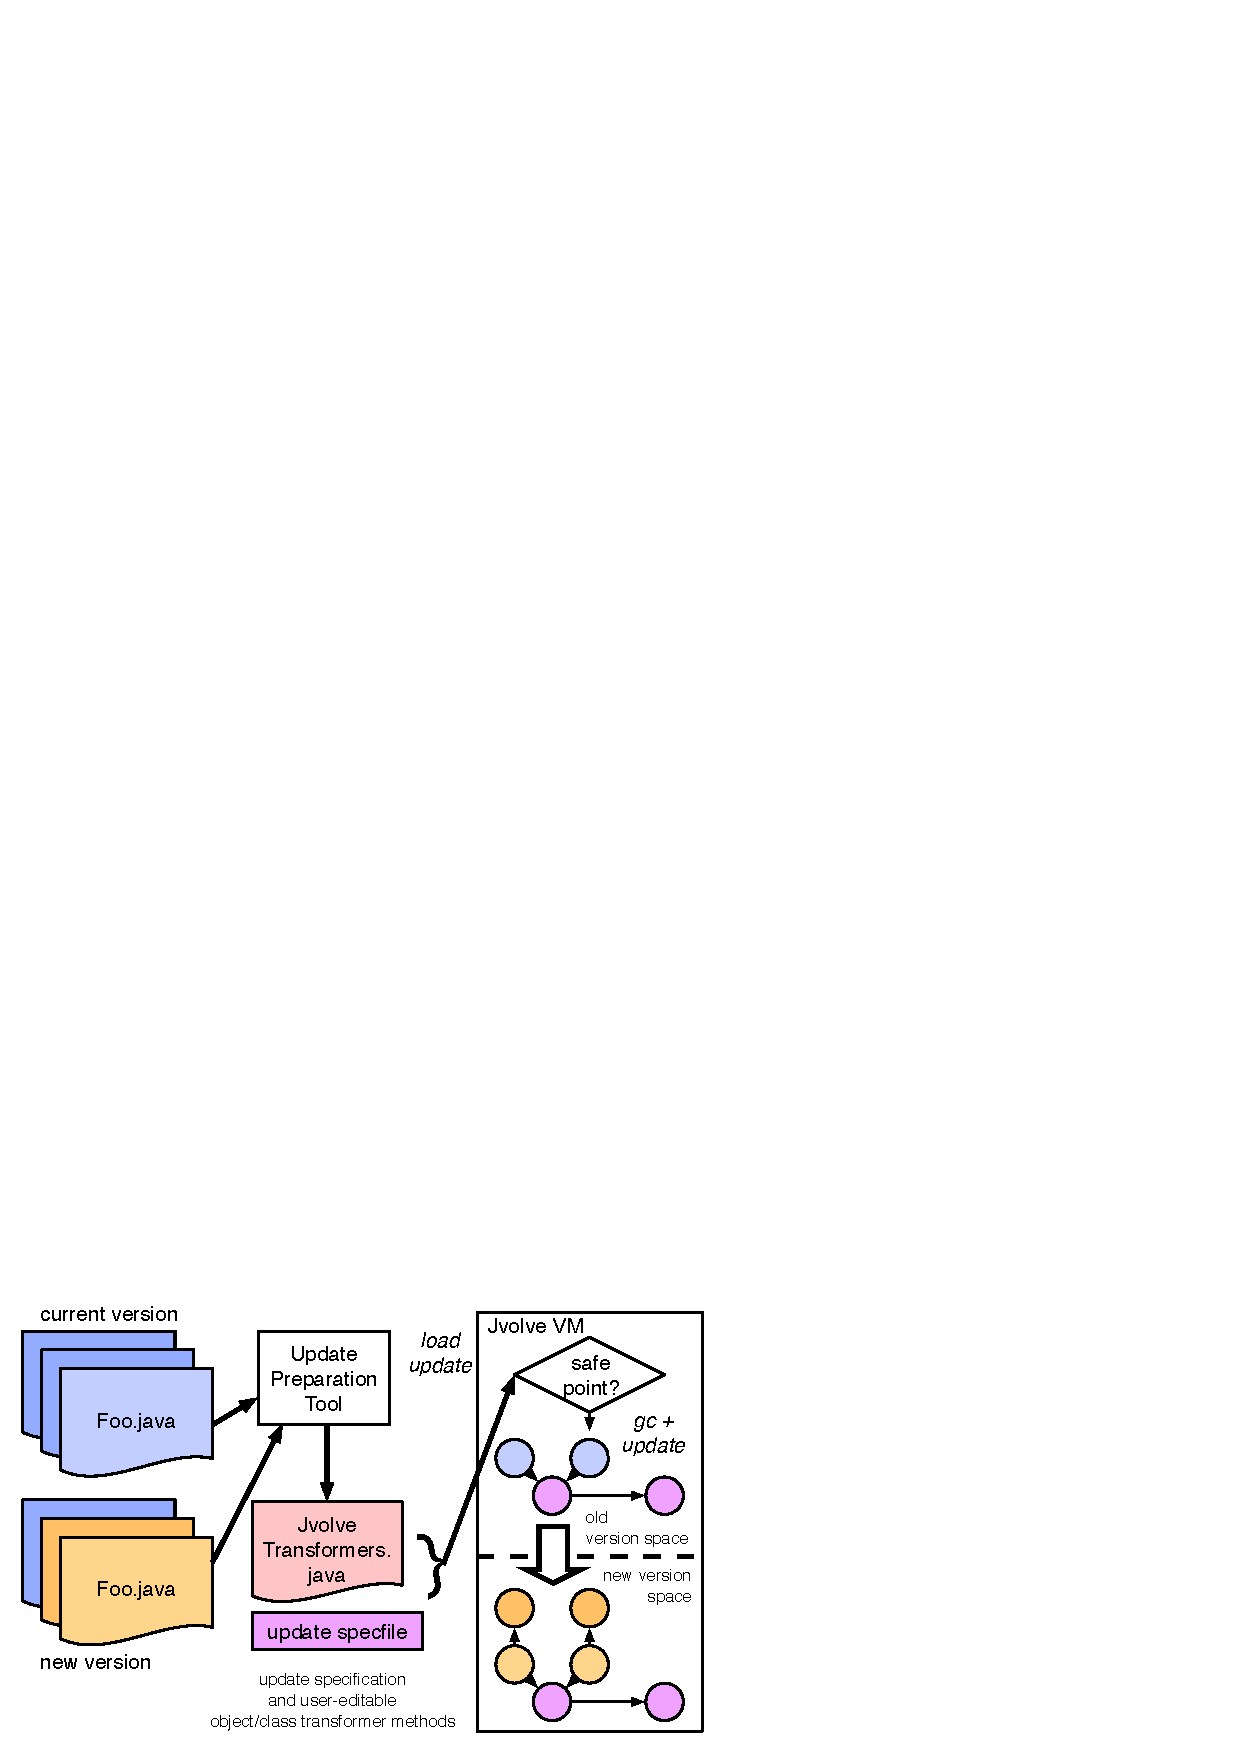
\includegraphics[width=0.84\paperwidth]{system.pdf}
\end{center}
\end{frame}

\begin{frame}{DSU Model}%{A Sub-title is optional}
\begin{itemize}
\item Old code and data before update
\item New code and data after update
\item Referential consistency
\item Compare bytecodes of versions offline, provide a patch to the VM
\item VM stops the application, performs the update, resumes with the new
version
\end{itemize}
\end{frame}

\begin{frame}{Implementation details}%{A Sub-title is optional}
\begin{itemize}
\item A lot of changes to the VM (that you do not want to know)
\item Currently using a Semi-Space Copying collector. Transform objects
during the copy
\item Support updates to three programs -- Jetty webserver,
JavaEmailServer, CrossFTPServer
\end{itemize}
\end{frame}

\begin{frame}{What's left in the implementation?}%{A Sub-title is optional}
\begin{itemize}
\item Better multiprocessor support
\item Leverage On-Stack Replacement (OSR) to support changes to active
methods on stack
\item Support changes with other GC models, specifically a concurrent
collector
\end{itemize}
\end{frame}

\begin{frame}{What's left in general?}%{A Sub-title is optional}
\begin{itemize}
\item Some formal/informal analysis about how safe DSU is
\item This is an undecidable problem. Restrict ourselves to what is
practical and useful
\item Support more applications
\end{itemize}
\end{frame}

\begin{frame}{Longer term}%{A Sub-title is optional}
\begin{itemize}
\item What other languages/applications need DSU support?
\item What about Python/Django, Ruby/RubyOnRails?
\item These languages are becoming more prevalent. On my laptop: 1698 ELF
files and 153 python files in /usr/bin directory 
\item Is it easier or harder for these languages? Is this an important
problem?
\end{itemize}
\end{frame}

\begin{frame}{Unrelated problem that I would like to be solved}%{A Sub-title is optional}
\begin{itemize}
\item Type checking: Static when possible, Dynamic when not (with type
inference)
\item Pain of typing in Java, versus the uncertainty of not knowing at
coding time if code is "even" type-correct in Python
\item A middle-ground between Java and Python (don't necessarily like this
approach)
  \begin{itemize}
  \item Static analysis for Python
  \item Supporting dynamic features in Java
  \end{itemize}
\end{itemize}
\end{frame}

\end{document}
